


% ######################################################################### %
% ------------------------------------------------------------------------- %
%                                Rewiring
% ------------------------------------------------------------------------- %
% ######################################################################### %


\section{Rewiring}

% In the network configuration introduced in
% section~\ref{sec:network_model} strong directional anisotropy is
% present: Edges originating from one node \enquote{point in the same
%   direction}, that is they connect to other nodes which cluster around
% a. In this section we introduce an algorithm

It is in our highest interest to compare results to. 
%------------------------------------------------
\marginpar{eliminate anisotropy through rewiring}
%------------------------------------------------ 
To this end we introduce an algorithm that preserves
distance-dependent connectivity as found in
Proposition~\ref{distance_prof}, but eliminates anisotropy in network
connectivity by consecutively rewiring existing connections to new
suitable targets.


\begin{definition}
Let $G$ be an anisotropic geometric graph with $\abs{V(G)} = n$. Then we define a
rewiring of $G$ to be probability space over $G^n_{\Phi}$, obtained by
choosing for every edge $e \in E(G)$ uniformly at random a potential new target $t'(e)$
from the set $M_e$ of all vertices that differ in their distance to
$s(e)$ less than $\varepsilon$ from the distance of $s(e)$ to $t(e)$,
\[
M_e =  \left\{v \in V(G) \setminus s(e) \mid \abs{\mathrm{d}(s(e),v) -
      \mathrm{d}(s(e),t(e))} < \varepsilon \right\}.
\]

\end{definition}


\begin{proposition}
Preserves distance-connectivity.
\end{proposition}

% for every neuron:
%    for every outgoing connection:
%        x = distance to target
%        new_targets = all nodes in distance $(x-\epsilon,x+\epsilon)$


\begin{remark}
Partial rewiring. $R_{\varepsilon, \eta}$
\end{remark} 

Here we choose $\varepsilon = ??$.

\vspace{0.2cm}
\begin{figure}[H]
  \centering 
  \makebox[0.875\textwidth]{%
    %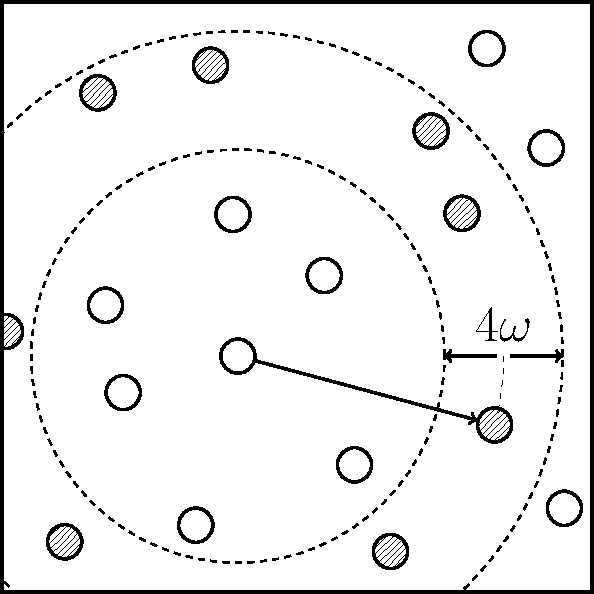
\includegraphics[width=0.4\textwidth]{dist_rew_org.pdf}%
    \begin{overpic}[width=0.4\textwidth, frame]{%
        tikz/distance_rewire_L3.pdf}
      \put(2,102){\small{Before}}
    \end{overpic}
    \hfill
    \begin{overpic}[width=0.4\textwidth, frame]{%
        tikz/distance_rewire_L4.pdf}
      \put(2,102){\small{After}}
    \end{overpic} 
  }%
  \caption{\textbf{Rewiring transforms anisotropic geometric graphs to
      networks with isotropic connectivity} For a given edge $e$ with
    a distance $x$ from its source vertex $v$ to its target vertex
    $t(e)$, potential new targets (striped) are found in within a
    distance $(x-\varepsilon, x+\varepsilon)$ of $v$. The rewired edge
    then projects from $v$ to a new target $t'(e)$, randomly chosen
    from the set of vertices within in this range. Inter-vertex
    distance between $v$ and $t'(e)$ differs by less than
    $\varepsilon$ from $x$, ensuring that for small $\varepsilon$ the
    original distance-dependent connectivity is preserved.}
  \label{fig:distance_rewiring}
\end{figure}

 

% \begin{algorithm}
% Let $N(n,e,w) = (G,P,a)$ be  Then 
% \normalfont
% \begin{algorithmic}%[1] <-- gives line numbers
% \For {$v \in V(N_G)$}
%   \For {$e \in E_{\textrm{out}}(v)$}
%      \State $x \gets \norm{N_P(v)-t(e)}$
%      \State $T \gets \{w \in V(N_G) \mid  x-\varepsilon \leq
%      \norm{N_P(v)-N_P(w)} < x+\varepsilon\}$
%      \State $t(e) \gets \textrm{choice} T$
%   \EndFor
% \EndFor

% \end{algorithmic}
% is defined.
% \end{algorithm}


%%% Local Variables: 
%%% mode: latex
%%% TeX-master: "../dplths_document"
%%% End: 
